\section{Combinatorial Optimization}

    \frame{\sectionpage}

    \begin{frame}{Classical problems}
      \large
      \begin{spacing}{1.5}
      \begin{itemize}
        \item Knapsack problem
        \item Minimum spanning tree
        \item Traveling salesman problem
        \item Set cover problem
        \item Matching problem
        \item Vehicle routing problem
        \item Facility Location Problem
        \item Production Scheduling Problem
      \end{itemize}
      \end{spacing}
   \end{frame}

   \begin{frame}{NP-complete}
     \begin{itemize}
       \item \textcolor{green}{P(PTIME)}

       It contains all decision problems that can be solved by a deterministic Turing machine using a polynomial amount of computation time, or polynomial time.
       \item \textcolor{green}{NP(Nondeterministic Polynomial time)}

       Class of computational decision problems for which a given yes-solution can be verified as a solution in polynomial time by a deterministic Turing machine.
       \item \textcolor{green}{NP-complete}

       Class of decision problems which contains the hardest problems in NP. Each NP-complete problem has to be in NP.
       \item \textcolor{green}{NP-hard}
       
       A problem H is NP-hard when every problem L in NP can be reduced in polynomial time to H.
       Class of problems which are at least as hard as the hardest problems in NP.
     \end{itemize}

   \end{frame}

   \begin{frame}{NP-complete}
     \centering
     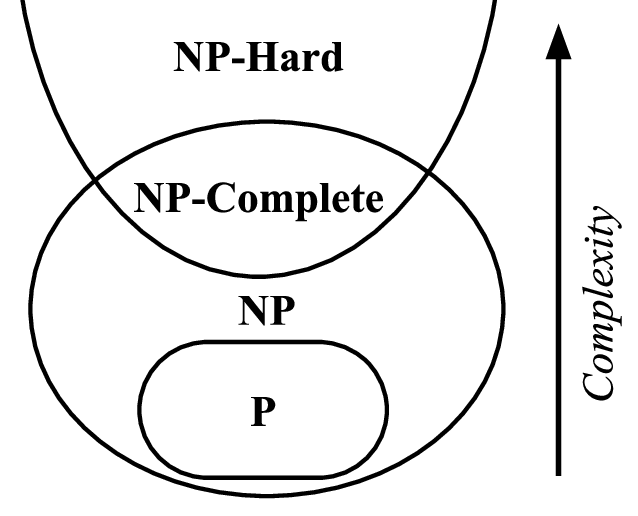
\includegraphics[width = 0.7\textwidth]{images/NP.png}
   \end{frame}

   \begin{frame}{How to solve Combinatorial optimization problem}
     \Large
     \begin{spacing}{1.5}
       \begin{itemize}
         \item Branch and bound
         \item Cutting plane
         \item Column generation
         \item ......
       \end{itemize}
     \end{spacing}
   \end{frame}


   \begin{frame}{Summary}
     Finally, we should master how to settle a problem in that way, so that we will have more ideas and try different methods.

     In the process of practice,they can guarantee to find the global solution, but in solving some typical practical problems, the price is too high, or it is easy to fall into local optimum. Because it's hard to accelerate the algorithm that can guarantee to find the optimal solution, that is, for most practical problems, it is difficult to find polynomial algorithm, because most of them are NP hard problems, then the rest selection is to design an algorithm that can jump out of local optimum.
   \end{frame}
